% !TEX encoding = UTF-8
% !TEX TS-program = pdflatex
% !TEX root = ../tesi.tex

%**************************************************************
\section{Sprint 3}
\label{sec:sprint3}
%**************************************************************
\subsection{User stories assegnate}
Anche se inizialmente era un'attività prevista per la quarta settimana ho iniziato a lavorare effettivamente al progetto durante il terzo sprint. \\
Utilizzando il documento precedentemente menzionato previste mi sono state assegnate le user stories da completare durante la settimana.
\noindent Ognuna di esse presenta i seguenti elementi:
\begin{itemize}
  \item nome della user story;
  \item un numero intero positivo che indica il ``peso'' in termini temporali che ci si aspetta che la user story abbia. Questi numeri seguono l'andamento della serie di Fibonacci e sono stati utili per allocare meglio le varie user stories all'interno degli sprint. Questi numeri vanno solitamente da 1 (task da meno di un'ora) a non più di 13 (task per il quale può essere necessaria fino a una settimana); 
  \item breve descrizione di ciò che si deve ottenere una volta conclusa la user story, dal punto di vista dell'utente;
  \item elenco di task, suddivisi tra frontend e backend, che dicono in modo più specifico e tecnico cosa fare per concludere la user story;
\end{itemize}
I quali verranno presentati nella forma:

\paragraph{Nome user story (Tempo previsto per concludere la user story)}\mbox{} \\[\baselineskip]
\noindent Descrizione dela user story. \\

\noindent Tasks:

\begin{itemize}
  \item Task1;
  \begin{itemize}
    \item subTask1;
  \end{itemize}
\end{itemize}
\vspace*{5pt}
\paragraph{Visualizzazione tabella (5)}\mbox{} \\[\baselineskip]
\noindent Come utente autenticato che si trova nella sezione “Reports”, voglio poter vedere la tabella riassuntiva delle ore spese. \\

\noindent Tasks:

\begin{itemize}
  \item implementare il componente principale della pagina Reports;
  \item implementare il componente della tabella, anche per quanto riguarda il suo stile;
  \item implementare la chiamata al backend per richiedere i dati da mostrare nella tabella;
  \item implementare la logica di query nel backend per soddisfare la richiesta dati.
\end{itemize}

\paragraph{Paginazione tabella (5)}\mbox{} \\[\baselineskip]
\noindent Come utente autenticato che si trova nella sezione “Reports”, voglio avere la tabella paginata, in modo da non avere troppe righe nella stessa schermata. \\

\noindent Tasks:

\begin{itemize}
  \item modificare la chiamata al backend già implementata per paginare i dati;
  \item aggiungere bottoni per passare da una pagina all'altra della tabella;
  \item aggiungere opzione per decidere quante righe includere in una pagina.
\end{itemize}

\subsection{Visualizzazione tabella}
\noindent Innanzitutto ho dovuto aggiungere all'applicazione la sezione Reports in quanto, seppure fosse già presente la tab per raggiungerla, non c'erano nè il percorso nè il componente della pagina.
A tal scopo ho aggiunto sia il percorso per raggiungere la sezione, \texttt{/reports}, al file contenente i routing privati dell'applicazione e ho creato il componente principale alla base della sezione Reports, per ora contenente solo il titolo.\\
Per permettere l'ottenimento dei dati, a lato frontend ho fatto uso di tre degli hooks che React già offre di base: \texttt{useState}, \texttt{useEffect} e \texttt{useCallback}, come nell'esempio di codice \ref{code:fetch}: \\
\begin{code}[frame=tb,label={code:fetch}, caption={Esempio di fetch dati da backend e memorizzazione in React state}]\\
1   const [data, setData] = useState([]);
2 
3   const fetchData = useCallback(async () => {
4     const resultData = await
5     /* Logica per la richiesta dei dati */
6     if (resultData) {
7       setData(resultData);
8     }
9    })
10
11  useEffect(() => {
12    fetchData();
13  }, [fetchData]);
\end{code}\\\\

\noindent \texttt{useEffect} indica che \texttt{fetchData} verrà chiamata dopo ogni rendering del componente, la quale otterrà i dati da mostrare in formato tabellare, che verranno salvati nel React state \texttt{data} tramite \texttt{useState}.
\texttt{useCallback} restituisce una funzione \texttt{fetchData} memoizzata, permettendo di non chiamarla nuovamente a ogni singolo re-rendering della pagina.\\
Per quanto riguarda la logica per la richiesta dei dati ho aggiunto un endpoint \texttt{/report} che risponde a una chiamata HTTP GET, ottenendo le \textit{attività} di un utente. Un'attività è un oggetto composto dai seguenti campi:
\begin{itemize}
  \item \texttt{id}: l'id univoco dell'attività;
  \item \texttt{user}
  \begin{itemize}
    \item \texttt{id}: l'id univoco dell'utente;
    \item \texttt{fullName}: il nome dell'utente;  
  \end{itemize}
  \item \texttt{project}
  \begin{itemize}
    \item \texttt{id}: l'id univoco del progetto a cui l'attività partiene;
    \item \texttt{name}: il nome del progetto;
  \end{itemize}
  \item \texttt{client}
  \begin{itemize}
    \item \texttt{id}: l'id univoco del cliente che commissiona il progetto;
    \item \texttt{name}: il nome del cliente;
  \end{itemize}
  \item \texttt{workspace}: il workspace dell'attività;
  \item \texttt{task}: il task che l'attività richiede;
  \item \texttt{work}: la durata in ore del'attività;
  \item \texttt{description}: breve descrizione dell'attività (opzionale);
  \item \texttt{day}: data in cui si è svolta l'attività;
  \item \texttt{workplace}: luogo in cui si è svolta l'attività.
\end{itemize}

Queste sono tutte le informazioni che la sezione report deve poter mostrare all'utente secondo i requisiti accordati.\\
L'endpoint \texttt{/reports} richiede inoltre dei query params aggiuntivi:
\begin{itemize}
  \item \texttt{from}: data prima della quale non si vuole nessuna attività;
  \item \texttt{to}: data dopo della quale non si vuole nessuna attività;
  \item \texttt{sort}: può assumere il valore 1 o -1. Nel primo caso i risultati della query saranno ordinati in modo ascendente, altrimenti in modo discendente;
  \item \texttt{token}: il token di accesso dell'utente.
\end{itemize}

A lato backend ho aggiunto la query per ottenere i dati da database.

Manca solo mostrare i dati e, a tal scopo, ho creato due nuovi React components, \texttt{ReportTable} e \texttt{ReportRow}.\\
Il primo racchiude la struttura della tabella, con tanto di header, mentre il secondo costituisce una riga della stessa. A seconda di quanti elementi saranno ottenuti dal backend, \texttt{ReportTable} chiamerà \texttt{ReportRow} un numero adeguato di volte, creando una tabella.

\subsection{Paginazone della tabella}

Ora la tabella è visibile, ma per evitare lunghi scroll verticali è necessario creare una funzionalità di paginazione, suddividendo quindi la tabella in parti più piccole, navigabili tramite una apposita interfaccia.\\
Sono possibili diverse implementazioni per una funzionalità di questo tipo, in particolare:
\begin{itemize}
  \item lato client, si richiedono tutti i dati con una sola chiamata, per poi mostrarne solo la quantità richiesta. Se l'utente vuole vedere altri dati è sufficiente prenderli da quelli già richiesti;
  \item lato server, si richiede una piccola quantità di dati, ad esempio solo 10 righe, che verranno poi mostrate. Se l'utente vuole vedere le successive 10 sarà necessario effettuare una nuova chiamata e poi mostrarle. 
\end{itemize}

In accordo con il team, ho optato per la seconda opzione in quanto si è deciso di dare priorità a non sovraccaricare troppo il client, anche perchè è facile arrivare ad avere centinaia se non migliaia di attività anche in periodi di tempo relativamente brevi. \\
Ho quindi aggiunto due React components:
\begin{itemize}
  \item \texttt{ReportTablePagination}: consiste in un menù a tendina che permette di scegliere quante righe la tabella potrà avere al massimo;
  \item \texttt{ReportTableNavigation}: consiste in un numero dinamico di bottoni che permettono le seguenti azioni:
  \begin{itemize}
    \item andare alla prima/ultima pagina;
    \item andare alla pagina precedente/successiva;
    \item andare a una pagina specifica.
  \end{itemize}
\end{itemize}

Al component principale \texttt{Report} ho aggiunto degli \texttt{useState} che permettono di implementare la funzionalità di paginazione:
\begin{itemize}
  \item \texttt{[maxRows, setMaxRows]}: controlla il numero massimo di righe impostato;
  \item \texttt{[currentPage, setCurrentPage]}: controlla la pagina in cui l'utente si trova al momento;
  \item \texttt{[totalRows, setTotalRows]}: controlla il numero totale di entry che sarebbero restituite dalla query senza paginazione.
\end{itemize}
Le prime due sono impostate dall'utente mentre per ottenere l'ultima è stato sufficiente aggiungere un campo \texttt{count} all'oggetto restituito dalla query precedentemente fatta. Sempre a questa query ho aggiunto due nuovi query params, calcolati lato client:
\begin{itemize}
  \item \texttt{skip}: quante entry ``saltare'' quando vado a richiedere le attività. Corrisponde a 0 se la pagina corrente è la prima, \texttt{currentPage - 1 * maxRows} altrimenti;
  \item \texttt{limit}: quante entry posso ottenere al massimo. Corrisponde a \texttt{maxRows}.
\end{itemize}

\subsection{Sprint review}
La sprint review si è conclusa in modo positivo, senza particolari correzioni necessarie. Anche i tempi sono stati rispettati.\\
La figura \ref{fig:report_table} mostra la tabella ottenuta e il relativo footer per navigarla e paginarla.

\begin{figure}[H]
	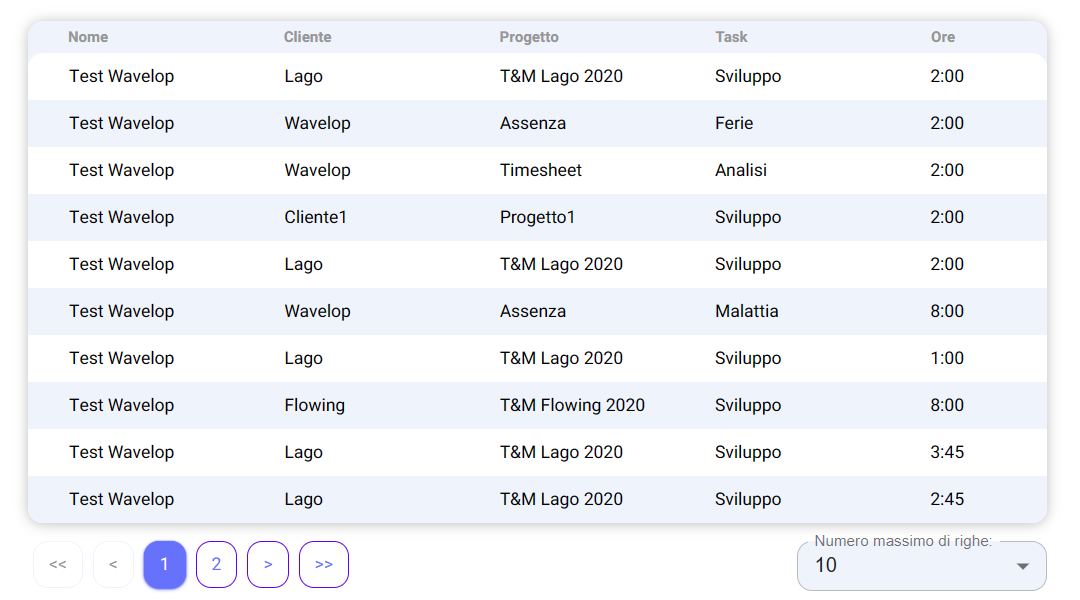
\includegraphics[width = \textwidth]{immagini/reports table.png}
	\caption{Tabella della sezione Reports}
	\label{fig:report_table}
\end{figure}